\begin{center}
	\zihao{4}\heiti
	% 中国科学院大学\\
	\LARGE{$\boldsymbol{2006}$年硕士学位研究生入学统一考试试题\\
	电动力学A卷}

\end{center}
\noindent
考生须知：\\
1.本试卷满分为150分,全部考试时间总计180分钟。\\
2.所有答案必须写在答题纸上,写在试题纸上或草稿纸上一律无效。

\vspace*{2ex}
\hrule
\vspace*{4ex} 

\fancypagestyle{mypagestyle}{%
	\fancyhf{}% Clear header/footer
	\fancyfoot[OR]{第~\thepage~页，共2页}%
	\fancyfoot[EL]{第~\thepage~页，共2页}%
	\fancyfoot[OL]{科目名称：电动力学 }%
	\fancyfoot[ER]{科目名称：电动力学 }%
	\renewcommand{\headrulewidth}{0pt}% Header rule of .4pt
	\renewcommand{\footrulewidth}{0.5pt}% Header rule of .4pt
}
\fancypagestyle{plain}{%
	\fancyhf{}% Clear header/footer
	\fancyfoot[OR]{第~\thepage~页，共2页}%
	\fancyfoot[EL]{第~\thepage~页，共2页}%
	\fancyfoot[OL]{科目名称：电动力学 }%
	\fancyfoot[ER]{科目名称：电动力学 }%
}

\setcounter{page}{1}%设置页面计数器
\pagestyle{mypagestyle}

\onehalfspacing
% 排版结束，下面是题目
\vspace{0.8cm}

\noindent
一、\hspace{0.8em}问答题（共25分，请写在答题纸上）

\noindent
1.\hspace{0.8em}写出非相对论形式的介质中麦克斯韦方程组的微分形式。

\noindent
2.\hspace{0.8em}写出平面电磁波在无限大均匀绝缘介质中的传播的特性。

\noindent
3.\hspace{0.8em}目前有两种类型的电子加速器，一类是直线型，一类是圆周型，在一定电磁作用力下两者的辐射功率与电子能量的关系分别是什么？因此目前能量较高的电子加速器一般采用哪种类型？

\vspace{0.4cm}
\noindent
二、\hspace{0.8em}选择题（共7题，每题5分，每一小题要求选取一个正确答案，请写在答题纸上）

\noindent
1.\hspace{0.8em}在自由面电荷两侧：\vspace{0.2cm}

(a)\hspace{0.6em}电势和电势的法向微分都是连续的；

(b)\hspace{0.6em}电势和电势的法向微分都不是连续的；

(c)\hspace{0.6em}电势是连续的，而电势的法向微分不是连续的；

(d)\hspace{0.6em}电势不是连续的，而电势的法向微分是连续的；
\vspace{0.2cm}

\noindent
2.\hspace{0.8em}在两个夹角为$\ang{90}$的接地导体平板之间有一点电荷q，用电象法求解此区间的电场时，其象电荷的数目为：\vspace{0.2cm}

(a)\hspace{0.6em}一个\hspace{1.6em}(b)\hspace{0.6em}两个\hspace{1.6em}(c)\hspace{0.6em}三个\hspace{1.6em}(d)\hspace{0.6em}四个
\vspace{0.2cm}

\noindent
3.\hspace{0.8em}如果一个矩形空腔波导管内填满了相对介电常数为$\large{\boldsymbol{\varepsilon_r}}$的电介质，那么其截止频率$\large{\boldsymbol{\omega_d}}$与原没有填充介质的空腔的截止频率$\large{\boldsymbol{\omega_0}}$之间的关系为：（角标d和0分别表示电介质和真空）

\vspace{0.4cm}
(a)\hspace{0.6em}$\large{\boldsymbol{\omega_d} = \boldsymbol{\varepsilon_r} \boldsymbol{\omega_0}}$\hspace{1.6em}(b)\hspace{0.6em}$\large{\boldsymbol{\omega_d} = \displaystyle{\frac{1}{\boldsymbol{\varepsilon_r}}} \boldsymbol{\omega_0}}$\hspace{1.6em}(c)\hspace{0.6em}$\large{\boldsymbol{\omega_d} = \sqrt{\boldsymbol{\varepsilon_r}} \boldsymbol{\omega_0}}$\hspace{1.6em}(d)\hspace{0.6em}$\large{\boldsymbol{\omega_d} = \displaystyle{\frac{1}{\sqrt{\boldsymbol{\varepsilon_r}}}} \boldsymbol{\omega_0}}$
\vspace{0.4cm}

\noindent
4.\hspace{0.8em}海水电导率约为4(欧姆)$^{-1}$，已知海水的$\large{\boldsymbol{\mu_r}}= 1$ , $\large{\boldsymbol{\mu_0}}= 4\large{\pi}$ $ \times 10^{-7} $享/米，则波长为3000米的无线电波在海水中的透入深度为：

\vspace{0.3cm}
(a)\hspace{0.6em}$\displaystyle{ \frac{ 3 }{4 \large{\boldsymbol{\pi}} } }$米 \hspace{1.6em}(b)\hspace{0.6em}$\displaystyle{ \frac{ 5 }{ 2 \large{\boldsymbol{\pi}}} }$米\hspace{1.6em}(c)\hspace{0.6em}$\displaystyle{ \frac{ 2 }{ 5 \large{\boldsymbol{\pi}}} }$米\hspace{1.6em}(d)\hspace{0.6em}$\displaystyle{ \frac{ 4 }{ 3 \large{\boldsymbol{\pi}}} }$米
\vspace{0.3cm}

\noindent
5.\hspace{0.8em}自然光以布儒斯特角入射到玻璃板上，
\vspace{0.2cm}

(a)\hspace{0.6em}反射光为完全偏振光\hspace{4.5em} (b)\hspace{0.6em}折射光为完全偏振光

(c)\hspace{0.6em}反射光为自然光\hspace{6.6em} (d)\hspace{0.6em}折射光为自然光
\vspace{0.2cm}

\noindent
6.\hspace{0.8em}若有一边长为$\rm{L}$的立方体，均匀带电，总电量为$\rm{Q}$，坐标原点在该立方体内中心处，其：
\vspace{0.2cm}

(a)\hspace{0.6em}电偶极矩和电四极矩均与$Q^2$有关

(b)\hspace{0.6em}电偶极矩为0，电四极矩不为0

(c)\hspace{0.6em}电偶极矩不为0，电四极矩为0

(d)\hspace{0.6em}电偶极矩，电四极矩均为0

\newpage
\noindent
7.\hspace{0.8em}如图，一单位面元的法线矢量为$\large{\boldsymbol{\Vec{d\sigma}}}$与电场$\large{ {\Vec{E}}}$的夹角为$\ang{30}$，当$\large{ {\Vec{B}}}=0$，$\large{ {\Vec{E}}} \neq 0$时，作用在该面元$\large{\boldsymbol{\Vec{d\sigma}}}$的电场力$\large{\boldsymbol{\Vec{df_E}}}$与$\large{\boldsymbol{\Vec{d\sigma}}}$的夹角为：\vspace{0.2cm}

(a)\hspace{0.6em}$\ang{90}$\hspace{9em}(b)\hspace{0.6em}$\ang{15}$

\vspace{0.2cm}
(c)\hspace{0.6em}$\ang{30}$\hspace{9em}(d)\hspace{0.6em}$\ang{60}$
\vspace{-2.4cm}

\begin{figure}[h]
    \flushright
    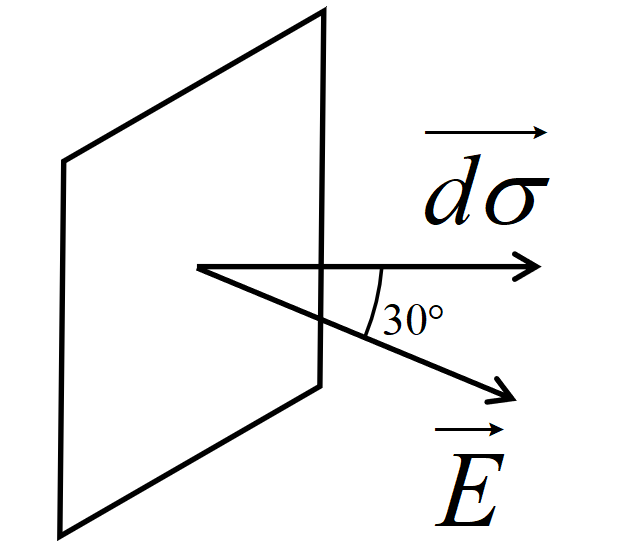
\includegraphics[height=2.4cm]{test/2006/pic_1.png}
        \label{fig:2006A_1}
\end{figure}

\noindent
三、\hspace{0.8em}（20分）一巨大平行电容板的两极板之间，充满介电系数为$\large{\boldsymbol{\varepsilon}}$的电介质，（可不考虑边缘效应），已知电容器两极板内表面上的电荷密度分别为$\large{\boldsymbol{+\sigma}}$和$\large{\boldsymbol{-\sigma}}$，在介质内部有一球状真空空隙，半径为$\large{ {R_0}}$，球心为$\large{\boldsymbol{O}}$点。求球内外的电势。
\vspace{-0.5cm}
\begin{figure}[h]
    \flushright
    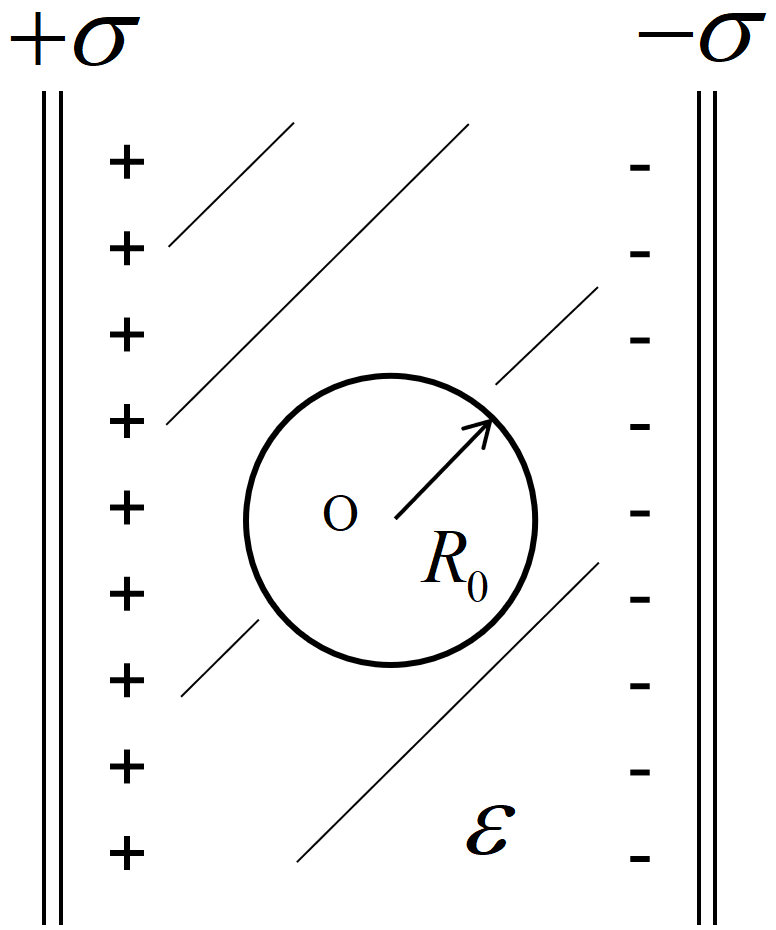
\includegraphics[height=3.5cm]{test/2006/pic_2.png}
        \label{fig:2006A_2}
\end{figure}

\noindent
四、\hspace{0.8em}（20分）真空中，有$q(0,0,0), q(0,0,2a), -2q(0,0,a)$沿z轴排列，彼此间的距离为a，求:

\noindent
1.\hspace{0.6em}该电荷体系的电偶极距和电四极距

\noindent
2.\hspace{0.6em}该电荷体系在距离原点$R$处$(R \gg a)$的电势，精确到四极矩项

\vspace{-1.2cm}
\begin{figure}[h]
    \flushright
    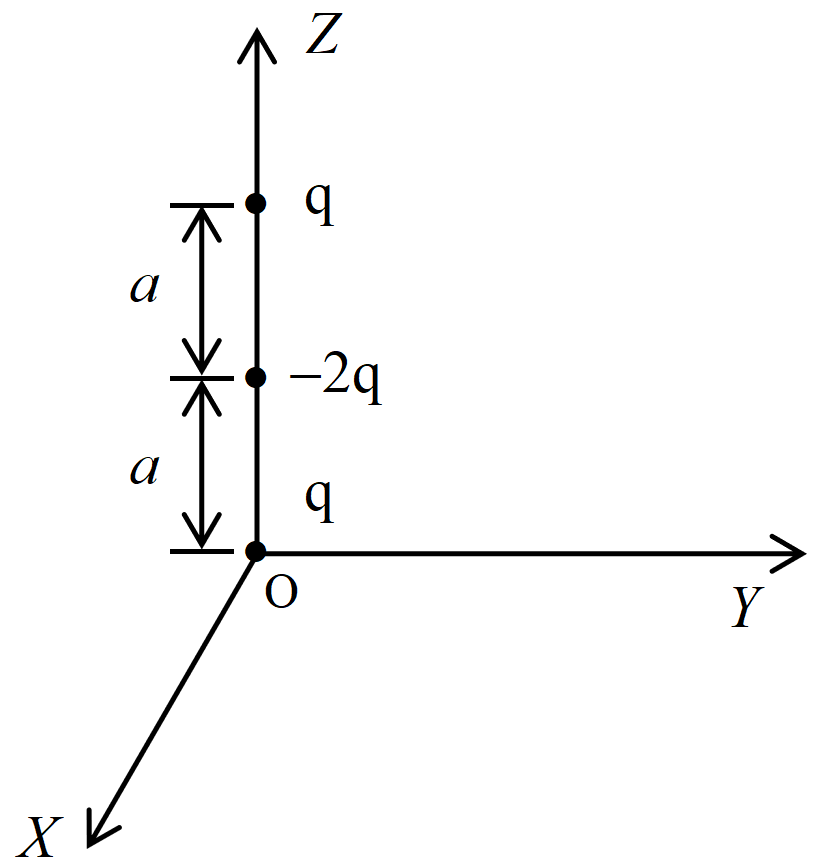
\includegraphics[height=4cm]{test/2006/pic_3.png}
        \label{fig:2006A_3}
\end{figure}

\noindent
五、\hspace{0.8em}（20分）有一带电粒子q沿z轴做简谐振动$z = z_0 e^{-i\omega t}$，设$z_0 \boldsymbol{\omega} \ll c$，试求，它在$r \gg \boldsymbol{\lambda}$处的辐射场的电场强度，磁感应强度，平均能流密度和辐射的总功率
\vspace{1.6cm}

\noindent
六，\hspace{0.8em}（20分）地面上同一地点发生两事件，其时间间隔为3秒，现有一高速运动的火箭，在火箭上的观察者观察此两件事发生的时间间隔为5秒（次序未变）
求：

\noindent1.\hspace{0.6em}此火箭相对于地面的速度是多少？

\noindent2.\hspace{0.6em}对火箭上的观察者来说，此两事件的空间距离是多少？
\vspace{1.6cm}

\noindent
七、\hspace{0.8em}（10分）如图所示，在空气中一根通以电流I的长直导线平行于半无限的软铁磁材料表面，与该表面的距离为a，软铁磁材料的$\boldsymbol{\mu}$可视为$\infty$，求：空气中P点处的磁场强度$\vec{H}$

\begin{figure}[h!]
    \flushright
    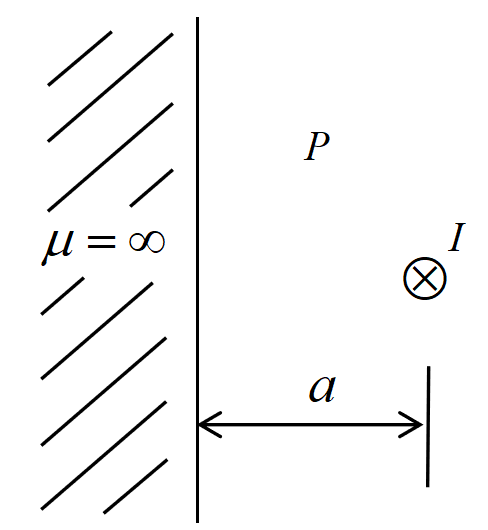
\includegraphics[height=3.2cm]{test/2006/pic_4.png}
        \label{fig:2006A_4}
\end{figure}
